% !TeX spellcheck = en_US
% !TeX encoding = UTF-8
% !TeX root = ../document.tex

\chapter{A Fast Search Algorithm}

\section{Concept}
The basic idea behind the \emph{Quickscan} algorithm is to select interesting regions as RoI (region of interest) candidates and discard most other regions, before the actual \p~value calculation.
This is done by evaluating a less computation intensive estimator over all possible connected regions, and making a selection of the most significant deviations according to this estimator. Finally, the full \p~value and its integral are only calculated for the few candidate regions returned by the estimator.

%\section{Components}
%This chapter will describe additional complications that have been encountered during the development of the Quickscan algorithm and propose implemented solutions to each of them.

\subsection{The Estimator}
The choice of the estimator plays an important role in the efficiency of the selection. A commonly used quantity in particle physics is 
\begin{equation}
\mychi = \frac{|\Ndata - \Nmc|}{\sigmamc'}
\end{equation}
Here the value $\sigmamc'$ describes the expected deviation. This is not $\sigmamc$, because that value only includes systematic uncertainties, e.g. finite Monte-Carlo statistics, and has been scaled by the luminosity.
$\sigmamc'$ consists of the expected statistical deviation $\sqrt{\Nmc}$ and the systematical error $\sigmamc$. The two errors are added quadratically. Because $\Nmc \geq 0$, the expression can be simplified:
\begin{equation}
\sigmamc' \defeq \sqrt{\sigmamc^2 + \left(\sqrt{\Nmc}\right)^2} = \sqrt{\sigmamc^2 + \Nmc}
\end{equation}

This value incorporated into the \mychi-value gives
\begin{equation}
\mychi = \frac{|\Ndata - \Nmc|}{\sqrt{\sigmamc^2 + \Nmc}}
\end{equation}

\subsection{Selection}
In each distribution, the \mychi~value is calculated for each connected bin region. The most significant regions are stored in a list. This introduces a parameter of the Quickscan algorithm, \paramregions, which denotes the number of candidates kept in the list.

\subsection{Nested Region Handling}
Using only the estimator and the selection of top \paramregions candidates, the algorithm tends to get stuck around single data points in the tail of the distribution. This is illustrated in figure \ref{fig:no_nested_region_handling}. 
\begin{figure}[htb]
	\centering
	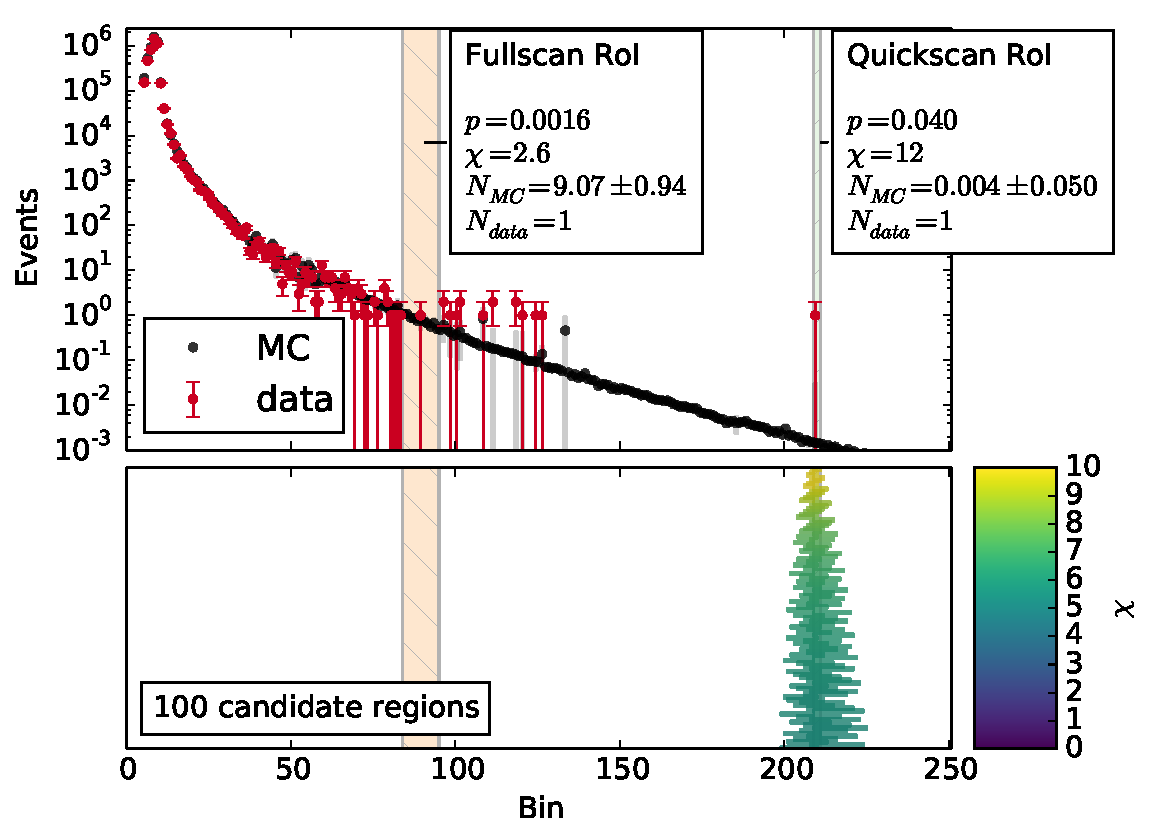
\includegraphics{no_nested_region_handling}
	\caption{Example distribution: pseudo experiment of the \eventclass{2e} \sumpT distribution, without special treatment of nested regions. The upper panel shows the distribution with the bin number (not the physical quantity) on the horizontal axis and the number of events in each bin on the vertical axis. The lower panel shows the 100 selected candidate regions, sorted by \mychi. The regions chosen by the different approaches are indicated in the upper panel. One can see that especially in the regions with 0-3 expected events, where the Poissonian approach $\sigma_N = \sqrt{N}$ fails, the \mychi value is too sensitive. The nested regions suppress different regions in the candidate list, such that the "true" RoI (as found without the Quickscan) is not detected.}
	\label{fig:no_nested_region_handling}
\end{figure}
The pseudo experiment of the \eventclass{2e} \sumpT distribution shows a single event above a low background expectation. The regions with the highest \mychi gather around this excess. Comparison with the full scan shows that the "true" region of interest is found further left in the distribution, as a deficit with only 1 observed event in 9 expected.

To suppress this behavior, an additional list of criteria is introduced, comparing region $A$ with region $B$:
\begin{my_list}
	\item $A$ is nested inside of $B$
	\item excess of data in $A$: $\Ndata(A) > \Nmc(A)$
	\item excess of data in $B$: $\Ndata(B) > \Nmc(B)$
	\item no additional data in $B \setminus A$: $\Ndata(A) = \Ndata(B)$
\end{my_list}
If all these conditions are met, then region $A$ is more significant than region $B$.
The conditions can be motivated as follows: if a region contains an excess of observed event yield over MC event yield, and the region is extended while the amount of observed event remains the same, the difference between \Nmc and \Ndata is reduced. Since the error \sigmamc can only increase, the total significance of the extended region must be less than the original region, as long as it still contains an excess.

\begin{figure}[htb]
	\centering
	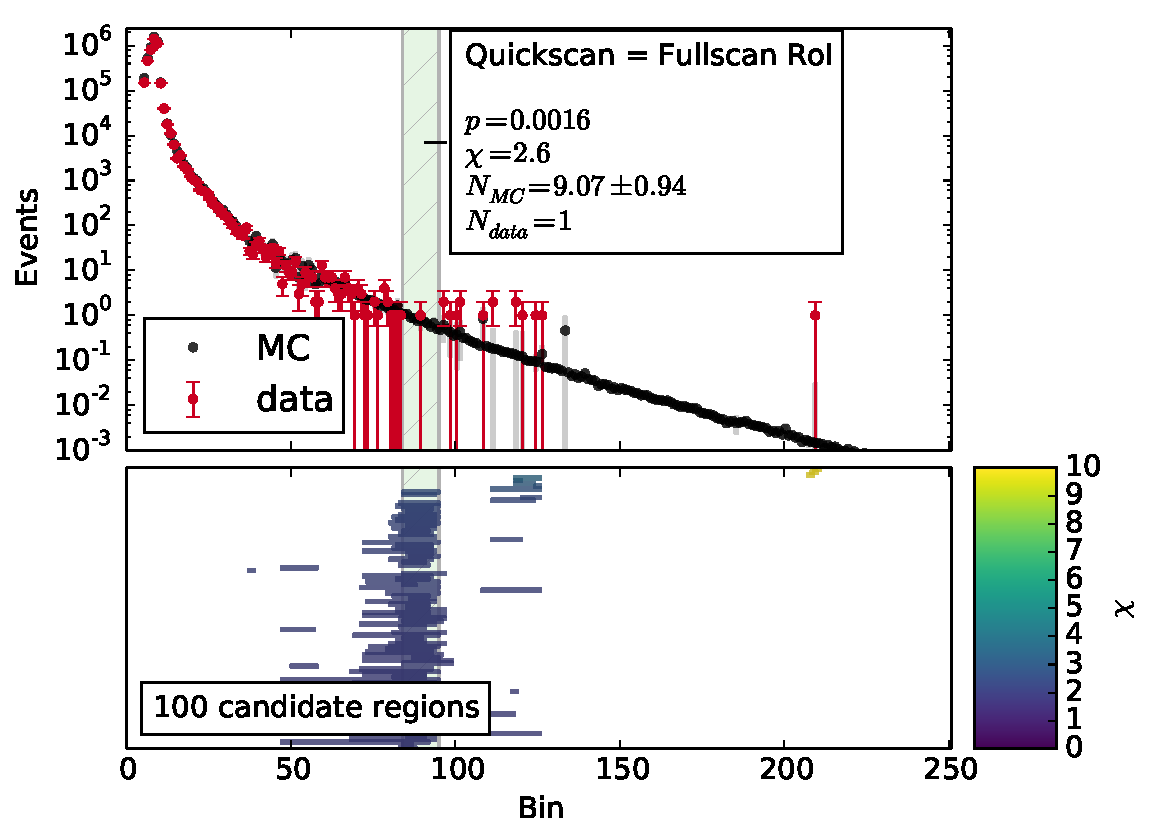
\includegraphics{with_nested_region_handling}
	\caption{Example distribution: pseudo experiment of the \eventclass{2e} \sumpT distribution, with special treatment of nested regions. The scheme is explained below figure \ref{fig:no_nested_region_handling}. }
	\label{fig:with_nested_region_handling}
\end{figure}
Based on this comparison, regions are immediately rejected if a more significant subregion is already included in the candidate list. The results of this treatment can be observed in figure \ref{fig:with_nested_region_handling}. The distribution is exactly the same as in \ref{fig:no_nested_region_handling}, but the algorithm does not focus overly on the event in the tail, leading to the correct RoI to be found.

%\subsection{Magnitude Binning}
%Ideally, the estimator should indicate significance in the same way as the \p~value. For this to work, there should be a monotonous functional dependency $\p(\mychi)$. To investigate this, one can plot \mychi vs. \p (figure \ref{fig:pvschi_vary_data}). In this illustration, \Nmc and \sigmamc are set to fixed values and \Ndata is varied. 
%\begin{figure}[htb]
%	\centering
%	\includegraphics{pvschi_vary_data}
%	\caption{Dependency of the \mychi~value and the \p~value. No physics data is involved, instead the value \Nmc and \sigmamc have been fixed and the amount of data \Ndata was varied in integer steps. With an optimal estimator, there should be no dependency on \Nmc, and all lines should align on top each other, with \mychi monotonically decreasing with \p.}
%	\label{fig:pvschi_vary_data}
%\end{figure}
%
%The first conclusion that can be drawn from this plot is that there is no trivial dependency $\p(\mychi)$. The significance expression depends on \Nmc, such that the best dependency can be $\p(\mychi, \Nmc, \sigmamc)$.
%A second conclusion is that for a fixed value of \Nmc, the dependency is monotonous. Thus, when comparing regions with the same value of \Nmc, \mychi is a valid indicator for significance which could be directly related to \p.
% 
%These conclusions motivate a solution called \emph{magnitude binning}.
%In order to only compare regions with approximately the same \Nmc, Quickscan first determines the magnitude $\log(\Nmc)$. For each magnitude, a separate list of \paramregions regions is maintained. 
%The index $i$ of each bin is calculated as 
%\begin{equation}
%i = \floor{\log_\parambinbase(\Nmc)} = \floor{\frac{\log(\Nmc)}{\log(\parambinbase)}}
%\end{equation}
%Here, a new parameter of the Quickscan algorithm, \parambinbase, has been introduced. It controls the size of the magnitude bins.
%
%\subsection{Separation of Excesses and Deficits}
%Figure \ref{fig:pvschi_vary_data} also shows that for a constant magnitude of \Nmc, $\p(\chi)$ has two branches which correspond to excesses and deficits. Because of this, each magnitude bin is again split into two separate candidate lists containing \paramregions regions each.

\section{The Final Algorithm}
The solutions suggested in this chapter are combined in the final algorithm: the Quickscan algorithm maintains a single list of \paramregions candidates for each distribution in each class. Everytime a new candidate is considered for insertion into the list, first the nested region criteria are evaluated. If the region is not nested inside any other region in the list, its \mychi~value is evaluated and compared to the list. If it is larger than the lowest \mychi inside the list, the region is swapped into the list.

After all regions have been considered, the \p~value is evaluated for all collected candidates and the final region of interest is determined. 

\section{Preserving the \p~Value of Data}
The Quickscan is only applied when the RoI of pseudo-experiments is calculated. Calculation of the \p~value of a data distribution is performed without the Quickscan algorithm.



